\documentclass[10pt,a4paper]{article}
\usepackage[margin=1.15cm]{geometry}
\usepackage{graphicx}
\usepackage{booktabs}
\usepackage{array}
\usepackage{xcolor}
\usepackage{hyperref}
\pagestyle{empty}

\definecolor{accent}{HTML}{1F4E79}
\definecolor{soft}{HTML}{F2F5F8}

\begin{document}

\begin{center}
{\Large\bfseries AI4Math: Scientific Computing and Mathematical AI Portfolio}\\[2pt]
{\small Python, PyTorch, C/C++, LaTeX, Jupyter, PyVista/VTK \quad | \quad 2026}
\end{center}

\vspace{-4pt}
\noindent
\colorbox{soft}{%
\begin{minipage}{0.97\linewidth}
\textbf{Project positioning.}
A course-based computational mathematics portfolio demonstrating practical
preparation for research assistant work: deep-learning experiments, numerical
simulation, scientific visualization, reproducible reports, and transparent
AI-assisted development.
\end{minipage}}

\vspace{8pt}
\begin{minipage}[t]{0.52\linewidth}
\raggedright
\textbf{\color{accent}Selected technical evidence}
\begin{itemize}\setlength\itemsep{2pt}
  \item Implemented PyTorch image-learning pipelines on MNIST-family datasets,
  including MLP/CNN baselines and AE/DAE/VAE latent-space visualizations.
  \item Built numerical computing modules in C/C++ and Python, including sparse
  CRS operations, LU/Poisson solver demos, and convergence checks.
  \item Created scientific visualization demos using Jupyter, PyVista, and VTK,
  including MRI slicing, terrain rendering, molecule density, and weather fields.
  \item Completed a celestial-mechanics final project with N-body integration,
  cached JPL Horizons validation, lunar flyby modeling, launch-window search,
  sensitivity analysis, and a reproducible LaTeX report.
\end{itemize}

\vspace{3pt}
\textbf{\color{accent}Representative deliverables}
\begin{itemize}\setlength\itemsep{2pt}
  \item \texttt{final\_project/Qian/report.pdf}
  \item \texttt{final\_project/Qian/README.md}
  \item \texttt{week11/experiments.md}
  \item \texttt{week13/outputs/opendx\_cases/case4\_mri\_slices.png}
\end{itemize}
\end{minipage}
\hfill
\begin{minipage}[t]{0.45\linewidth}
\raggedright
\textbf{\color{accent}RA-relevant skills}
\begin{tabular}{@{}>{\bfseries}p{0.28\linewidth}p{0.64\linewidth}@{}}
Programming & Python, C/C++, Git, Makefile workflows \\
ML/AI & PyTorch, CNNs, autoencoders, experiment logging \\
Numerics & N-body dynamics, RK4, Verlet, sparse matrices \\
Visualization & matplotlib, PyVista, VTK, Jupyter \\
Writing & LaTeX reports, result tables, AI-use disclosure \\
\end{tabular}
\end{minipage}

\vspace{8pt}
\begin{center}
\begin{tabular}{cc}
\includegraphics[width=0.45\linewidth]{week11/results/latent_space_ae.png} &
\includegraphics[width=0.45\linewidth]{week13/outputs/opendx_cases/case4_mri_slices.png} \\
{\small Autoencoder latent-space visualization} &
{\small MRI slice visualization with PyVista/VTK} \\[5pt]
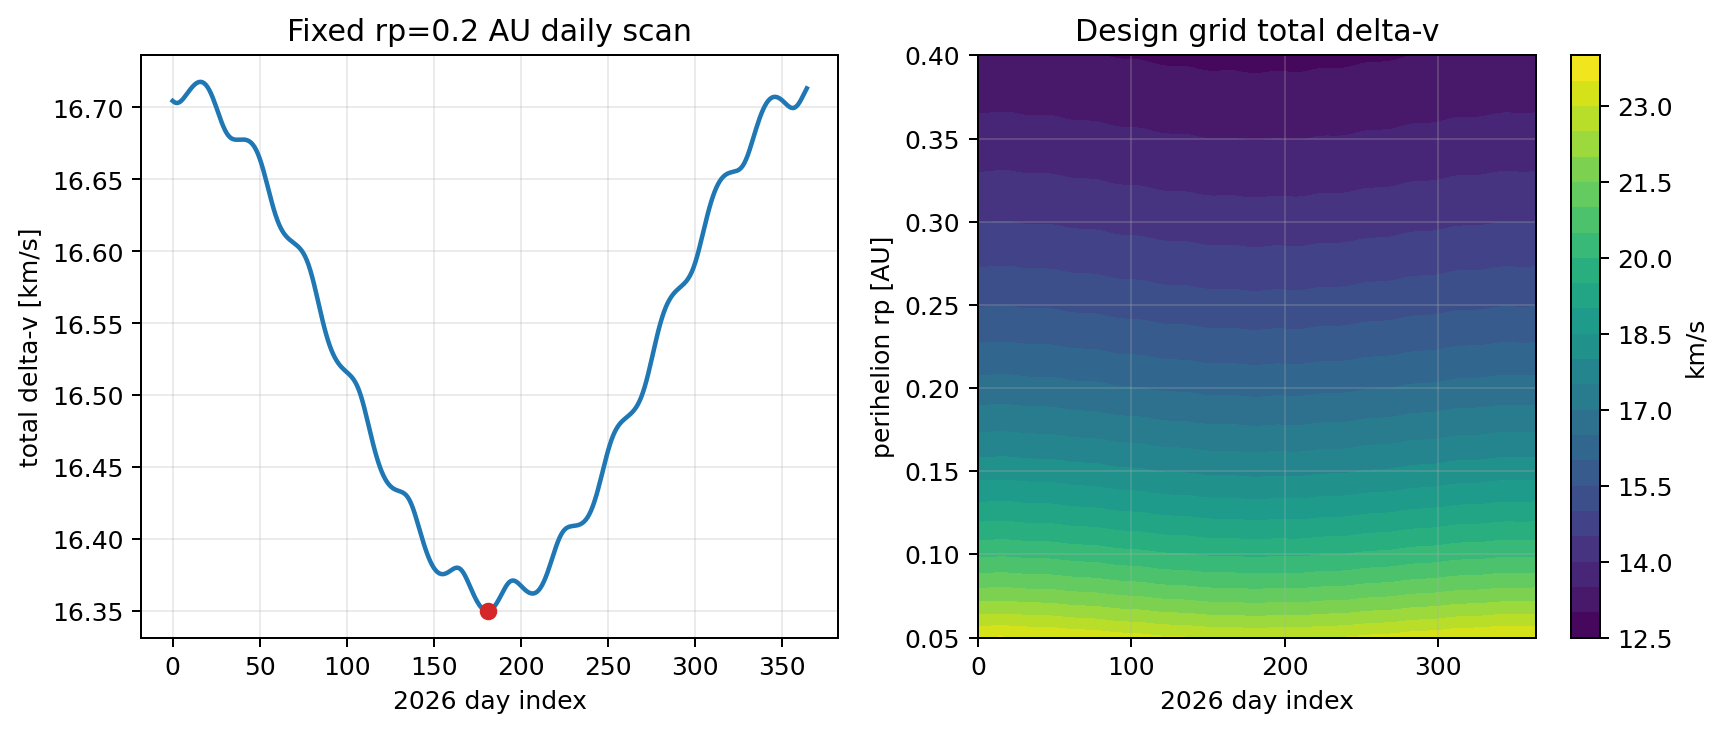
\includegraphics[width=0.45\linewidth]{final_project/Qian/figures/m6_launch_window.png} &
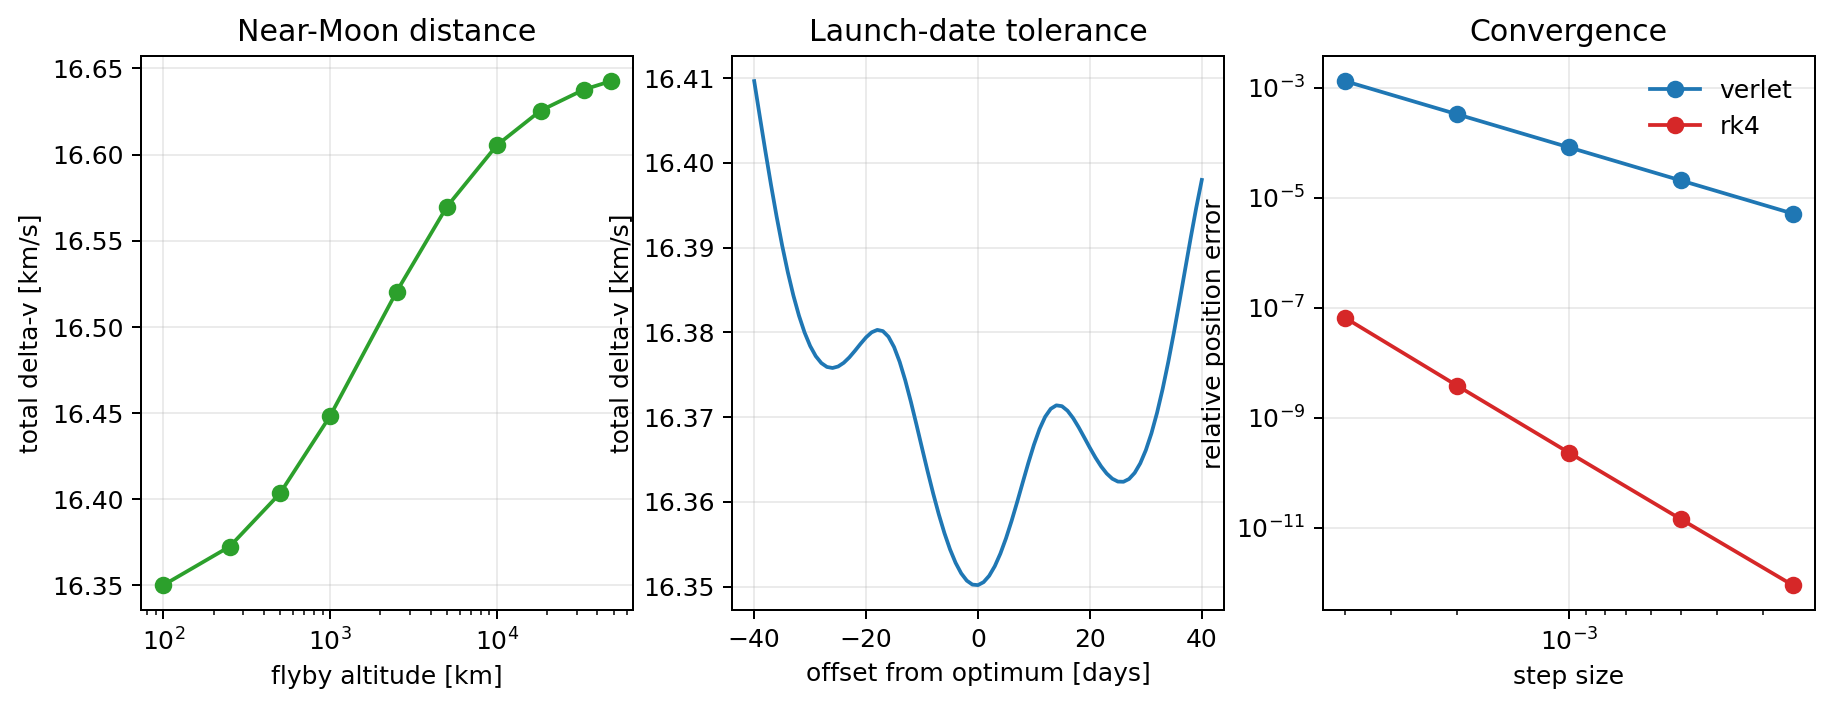
\includegraphics[width=0.45\linewidth]{final_project/Qian/figures/m7_sensitivity.png} \\
{\small 2026 launch-window scan} &
{\small Sensitivity and convergence analysis}
\end{tabular}
\end{center}

\vspace{-2pt}
\noindent
\textbf{\color{accent}Public-release note.}
Local credentials, private API tokens, temporary build files, executable
binaries, and cache directories are excluded or replaced with placeholders.

\end{document}
